%矢量点乘

% 这里只介绍几何矢量及对应的直角坐标列矢量
\pentry{几何矢量\upref{GVec}}

\subsection{几何定义}
我们先来看点乘的几何定义. 注意该定义不需要任何坐标系的概念.
\begin{figure}[th]
\centering
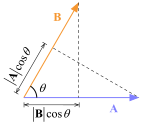
\includegraphics[width=5cm]{./figures/Dot1.pdf}
\caption{点乘的几何定义}\label{Dot_fig1}
\end{figure}

如\autoref{Dot_fig1}, 两个几何矢量的\bb{点乘(dot product)}\footnote{也叫\bb{点积},\bb{标量积(scalar product)}或\bb{内积(inner product)}}就是把它们的模长相乘,再乘以它们的夹角的余弦值.即
\begin{equation}\label{Dot_eq1}
\vec A \vdot \vec B = \abs{\vec A} \abs{\vec B} \cos\theta 
\end{equation}

其中 $\theta$ 是两个矢量的夹角. 注意两个矢量点乘得到的是一个标量. 几何定义中(\autoref{Dot_fig1}),既可以把点乘理解为 $\vec A$ 投影在 $\vec B$ 上的模长乘以 $\vec B$ 的模长,也可以理解为 $\vec B$ 投影在 $\vec A$ 上的模长乘以 $\vec A$ 的模长\footnote{在这种理解下,若量矢量的夹角为钝角,投影长度取负值}.可见当两矢量模长不变时,若方向相同,点乘取最大值 $\abs{\vec A}\abs{\vec B}$;若方向相反,点乘取最小值 $-\abs{\vec A}\abs{\vec B}$;若相互垂直,则点乘为 0.

我们说两个点乘为 0 的矢量互相垂直, 或者说\bb{正交}. 几何矢量与自身点乘可得该矢量模长的平方. 单位矢量与自己的点乘等于 1. 把一个矢量除以自身模长得到同方向单位矢量的过程叫做矢量的\bb{归一化}.

\subsection{点乘的性质}

\begin{enumerate}
\item \bb{交换律 \footnote{由\autoref{Dot_eq1} 易证}}
\begin{equation}\label{Dot_eq2}
\vec A \vdot \vec B = \vec B \vdot \vec A
\end{equation}

\item \bb{分配律 \footnote{证明见词条最后.}}
\begin{equation}\label{Dot_eq3}
\vec A \vdot (\vec B + \vec C) = \vec A \vdot \vec B + \vec A \vdot \vec C
\end{equation}
\end{enumerate}

注意点乘不满足结合律,即
\begin{equation}
(\vec A \vdot \vec B) \vec C \ne  \vec A (\vec B \vdot \vec C)
\end{equation}
前者是 $\vec C$ 方向的矢量,后者是 $\vec A$ 方向的矢量,显然不相等.

\subsection{点乘的坐标运算}
\pentry{正交归一基\upref{OrNrB}}
若已知 $\vec A, \vec B$ 在平面直角坐标系 $xy$ 中坐标分别为 $(A_x, A_y)$ 和  $(B_x, B_y)$,那么如何用坐标表示点乘运算的结果呢? 先用正交归一基\upref{OrNrB} 将两矢量展开 %未完成,矢量空间里面要介绍基底及坐标的唯一性.
\begin{equation}
\vec A = A_x \,\uvec x + A_y \,\uvec y \qquad \vec B = B_x \,\uvec x + B_y \,\uvec y
\end{equation}
所以
\begin{equation}
\vec A \vdot \vec B = (A_x \,\uvec x + A_y \,\uvec y) \vdot (B_x \,\uvec x + B_y \,\uvec y)
\end{equation}
根据分配律\autoref{Dot_eq3},我们可以把两个括号拆开,变为 4 个点乘之和. 
\begin{equation}
\vec A \vdot \vec B = A_x B_x \,\uvec x \vdot \uvec x + A_y B_y \,\uvec y \vdot \uvec y + A_x B_y \,\uvec x \vdot \uvec y + A_y B_x \,\uvec y \vdot \uvec x
\end{equation}
其中 $\uvec x \vdot \uvec y = \uvec y \vdot \uvec x = 0$ (相互垂直), 而 $\uvec x \vdot \uvec x = \uvec y \vdot \uvec y = 1$ (相互平行且模长都为1). 所以最后结果为
\begin{equation}
\vec A \vdot \vec B = A_x B_x + A_y B_y
\end{equation}
同理,可以在三维直角坐标系 $xyz$ 中把点乘结果用坐标表示
\begin{equation}
\vec A \vdot \vec B = A_x B_x + A_y B_y + A_z B_z	
\end{equation}
注意点乘的代数定义也可以拓展到更高维的情况甚至复数的情况, 即对于复数域的 $u_1, u_2, \dots, u_N$ 和 $v_1, v_2, \dots, v_N$,
\begin{equation}
\vec u \vdot \vec v = \sum_k u_k v_k
\end{equation}

注意虽然上式中的坐标取决于正交归一基底的选取, 但点乘的结果却与基底的选取无关. 这是因为点乘的几何定义是两个几何矢量间的几何性质, 与基底无关.

\begin{figure}[ht]
\centering
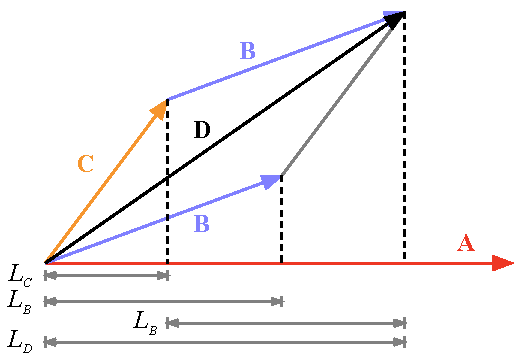
\includegraphics[width=8cm]{./figures/Dot2.pdf}
\caption{点乘分配律的证明} \label{Dot_fig2}
\end{figure}

\subsection{证明点乘的分配律}

如\autoref{Dot_fig2}, 令 $\vec D \equiv \vec B + \vec C$, 把 $\vec A \vdot \vec B$,  $\vec A \vdot \vec C$,  $\vec A \vdot \vec D$ 分别用几何定义理解为 $\vec B$,  $\vec C$,  $\vec D$ 在 $\vec A$ 上的投影乘 $\abs{\vec A}$, 且令投影长度分别为 $L_B, L_C, L_D$. 那么要证明 $\vec A \vdot (\vec B + \vec C) = \vec A \vdot \vec D = \vec A \vdot \vec B + \vec A \vdot \vec C$, 只需证明 $L_D = L_B + L_C$ 即可.现在把 $\vec B$ 平移使其起点与 $\vec C$ 的终点对接(投影长度不变). 从图中立即得出 $L_D = L_B + L_C$.  








